\documentclass{article} % For LaTeX2e
\usepackage{iclr2024_conference,times}

\usepackage[utf8]{inputenc} % allow utf-8 input
\usepackage[T1]{fontenc}    % use 8-bit T1 fonts
\usepackage{hyperref}       % hyperlinks
\usepackage{url}            % simple URL typesetting
\usepackage{booktabs}       % professional-quality tables
\usepackage{amsfonts}       % blackboard math symbols
\usepackage{nicefrac}       % compact symbols for 1/2, etc.
\usepackage{microtype}      % microtypography
\usepackage{titletoc}

\usepackage{subcaption}
\usepackage{graphicx}
\usepackage{amsmath}
\usepackage{multirow}
\usepackage{color}
\usepackage{colortbl}
\usepackage{cleveref}
\usepackage{algorithm}
\usepackage{algorithmicx}
\usepackage{algpseudocode}

\DeclareMathOperator*{\argmin}{arg\,min}
\DeclareMathOperator*{\argmax}{arg\,max}

\graphicspath{{../}} % To reference your generated figures, see below.
\begin{filecontents}{references.bib}
@article{lu2024aiscientist,
  title={The {AI} {S}cientist: Towards Fully Automated Open-Ended Scientific Discovery},
  author={Lu, Chris and Lu, Cong and Lange, Robert Tjarko and Foerster, Jakob and Clune, Jeff and Ha, David},
  journal={arXiv preprint arXiv:2408.06292},
  year={2024}
}

@book{goodfellow2016deep,
  title={Deep learning},
  author={Goodfellow, Ian and Bengio, Yoshua and Courville, Aaron and Bengio, Yoshua},
  volume={1},
  year={2016},
  publisher={MIT Press}
}

@article{vaswani2017attention,
  title={Attention is all you need},
  author={Vaswani, Ashish and Shazeer, Noam and Parmar, Niki and Uszkoreit, Jakob and Jones, Llion and Gomez, Aidan N and Kaiser, {\L}ukasz and Polosukhin, Illia},
  journal={Advances in neural information processing systems},
  volume={30},
  year={2017}
}

@article{karpathy2023nanogpt,
  title = {The Forward-Forward Algorithm: Some Preliminary Investigations},
  author = {Hinton, Geoffrey},
  year = {2022},
  journal = {arXiv preprint arXiv:2212.13345},
}

@article{kingma2014adam,
  title={Adam: A method for stochastic optimization},
  author={Kingma, Diederik P and Ba, Jimmy},
  journal={arXiv preprint arXiv:1412.6980},
  year={2014}
}

@article{ba2016layer,
  title={Layer normalization},
  author={Ba, Jimmy Lei and Kiros, Jamie Ryan and Hinton, Geoffrey E},
  journal={arXiv preprint arXiv:1607.06450},
  year={2016}
}

@article{loshchilov2017adamw,
  title={Decoupled weight decay regularization},
  author={Loshchilov, Ilya and Hutter, Frank},
  journal={arXiv preprint arXiv:1711.05101},
  year={2017}
}

@article{radford2019language,
  title={Language Models are Unsupervised Multitask Learners},
  author={Radford, Alec and Wu, Jeff and Child, Rewon and Luan, David and Amodei, Dario and Sutskever, Ilya},
  year={2019}
}

@article{journ2023hebbian,
  title={Hebbian Deep Learning Without Feedback},
  author={Journ\'e, Adrien and Garcia Rodriguez, Hector and Guo, Qinghai and Moraitis, Timoleon},
  journal={ICLR},
  year={2023}
}

@article{paszke2019pytorch,
  title={Pytorch: An imperative style, high-performance deep learning library},
  author={Paszke, Adam and Gross, Sam and Massa, Francisco and Lerer, Adam and Bradbury, James and Chanan, Gregory and Killeen, Trevor and Lin, Zeming and Gimelshein, Natalia and Antiga, Luca and others},
  journal={Advances in neural information processing systems},
  volume={32},
  year={2019}
}

@misc{gpt4,
  title={GPT-4 Technical Report},
  author={OpenAI},
  year={2024},
  eprint={2303.08774},
  archivePrefix={arXiv},
  primaryClass={cs.CL},
  url={https://arxiv.org/abs/2303.08774},
}

@Article{Pomerat2019OnNN,
 author = {John Pomerat and Aviv Segev and Rituparna Datta},
 booktitle = {2019 IEEE International Conference on Big Data (Big Data)},
 journal = {2019 IEEE International Conference on Big Data (Big Data)},
 pages = {6183-6185},
 title = {On Neural Network Activation Functions and Optimizers in Relation to Polynomial Regression},
 year = {2019}
}


@Article{He2015DelvingDI,
 author = {Kaiming He and X. Zhang and Shaoqing Ren and Jian Sun},
 booktitle = {IEEE International Conference on Computer Vision},
 journal = {2015 IEEE International Conference on Computer Vision (ICCV)},
 pages = {1026-1034},
 title = {Delving Deep into Rectifiers: Surpassing Human-Level Performance on ImageNet Classification},
 year = {2015}
}

\end{filecontents}

\title{Exploring Weight Initialization Strategies in Neural Networks: A Comparative Study}

\author{LLM\\
Department of Computer Science\\
University of LLMs\\
}

\newcommand{\fix}{\marginpar{FIX}}
\newcommand{\new}{\marginpar{NEW}}

\begin{document}

\maketitle

\begin{abstract}
This paper investigates the impact of various weight initialization strategies on neural networks trained using error diffusion learning, aiming to understand their effects on training dynamics, convergence speed, and final performance. Weight initialization is crucial yet challenging, as poor choices can lead to slow convergence or suboptimal solutions. We address this by implementing and comparing several strategies, including Xavier, He, uniform random, and normal distribution, within the \texttt{init\_network} function of a neural network. Our contribution includes a comprehensive evaluation across multiple datasets: XOR, Gaussian, spiral, and circle. We verify our approach through extensive experiments, tracking metrics such as training loss, accuracy, and time to convergence. Our results offer valuable insights into the effectiveness of each strategy, providing guidance for practitioners in selecting the most suitable method for their applications.
\end{abstract}

\section{Introduction}
\label{sec:intro}
Neural networks have become a cornerstone of modern machine learning, demonstrating remarkable performance across a wide range of tasks, from image recognition to natural language processing \citep{goodfellow2016deep}. However, the success of neural networks heavily depends on the initialization of their weights, which can significantly influence the training dynamics and final performance of the model. Poor initialization can lead to issues such as slow convergence, vanishing or exploding gradients, and suboptimal solutions \citep{kingma2014adam}. This paper investigates the impact of various weight initialization strategies on neural networks trained using error diffusion learning, a method that has shown promise in improving training efficiency and accuracy.

Understanding the effects of different weight initialization methods is crucial for designing efficient and effective neural networks. Weight initialization is a challenging problem because it directly affects the optimization process. For instance, initializing weights too small can lead to vanishing gradients, while too large weights can cause exploding gradients \citep{paszke2019pytorch}. This study aims to provide a comprehensive analysis of how different initialization strategies, including Xavier, He, uniform random, and normal distribution, affect the performance of neural networks on various datasets.

The challenge lies in selecting an appropriate initialization strategy that balances the trade-offs between convergence speed and final model performance. To address this, we implement several initialization strategies in the \texttt{init\_network} function of a neural network and evaluate their impact on training dynamics and performance. Our approach involves extensive experiments on multiple datasets, including XOR, Gaussian, spiral, and circle, to ensure the generalizability of our findings.

Our contributions are as follows:
\begin{itemize}
    \item We implement and compare several weight initialization strategies, including Xavier, He, uniform random, and normal distribution, in the context of error diffusion learning.
    \item We conduct extensive experiments on multiple datasets to evaluate the impact of these initialization strategies on training dynamics, convergence speed, and final performance.
    \item We provide insights and guidelines for practitioners on selecting the most appropriate weight initialization strategy for their specific applications.
\end{itemize}

To verify our approach, we track metrics such as training loss, accuracy, and time to convergence across different runs. Our results demonstrate the effectiveness of each initialization strategy, highlighting their strengths and weaknesses in various scenarios. These findings can guide practitioners in making informed decisions about weight initialization in neural network training.

While this study provides valuable insights, there are several avenues for future work. Exploring the impact of weight initialization in conjunction with other training techniques, such as batch normalization \citep{ba2016layer} and advanced optimization algorithms \citep{loshchilov2017adamw}, could further enhance our understanding of neural network training dynamics. Additionally, investigating the effects of weight initialization on more complex architectures and larger datasets would be beneficial.

\section{Related Work}
\label{sec:related}

The study of weight initialization strategies is crucial for understanding and improving the training dynamics of neural networks. Various methods have been proposed to address challenges such as slow convergence and vanishing/exploding gradients. This section reviews and compares the most relevant works, highlighting their contributions and limitations.

Xavier initialization aims to maintain the scale of gradients throughout the network by setting weights to values drawn from a distribution with zero mean and a specific variance. This method improves convergence speed and training stability, particularly in networks with sigmoid or tanh activation functions. Our findings align with these results, showing significant improvements in accuracy and convergence speed for certain datasets.

He initialization, introduced by \citet{He2015DelvingDI}, is designed for layers with ReLU activation functions. It sets weights to values drawn from a distribution with a variance inversely proportional to the number of input units, addressing vanishing gradients in deep networks with ReLU activations. Our experiments with He initialization showed mixed results, indicating its effectiveness may depend on the specific dataset and network architecture.

While our study focuses on weight initialization strategies, other works have explored different aspects of neural network training. For instance, \citet{kingma2014adam} proposed the Adam optimization algorithm, which combines the advantages of AdaGrad and RMSProp. Although Adam improves training efficiency, our study did not focus on optimization algorithms, as our primary goal was to evaluate the impact of weight initialization.

Batch normalization, introduced by \citet{ba2016layer}, normalizes the inputs of each layer to mitigate vanishing and exploding gradients. However, our experiments did not include batch normalization, as we aimed to isolate the effects of weight initialization on training performance.

Advanced optimization algorithms, such as AdamW \citep{loshchilov2017adamw}, incorporate weight decay regularization to prevent overfitting and improve generalization. While valuable, our study focused on the initialization phase, and future work could explore the interaction between weight initialization and advanced optimization algorithms.

In summary, while various methods have been proposed to improve neural network training, our study specifically addresses the impact of weight initialization strategies. By comparing and contrasting our findings with existing works, we provide a comprehensive understanding of the strengths and limitations of different initialization methods. Future research could build on our results by incorporating other training techniques, such as batch normalization and advanced optimization algorithms, to further enhance neural network performance.

\section{Background}
\label{sec:background}

Weight initialization is a critical aspect of training neural networks, significantly influencing convergence speed and final performance. Poor initialization can lead to vanishing or exploding gradients, hindering the optimization process \citep{goodfellow2016deep}. Various strategies have been proposed to address these challenges, including Xavier initialization and He initialization \citep{he2015delving}.

Xavier initialization, also known as Glorot initialization, aims to maintain the scale of gradients throughout the network by setting weights to values drawn from a distribution with zero mean and a specific variance, depending on the number of input and output units in the layer. He initialization, designed for layers with ReLU activation functions, sets weights to values drawn from a distribution with a variance inversely proportional to the number of input units \citep{He2015DelvingDI}.

Other strategies, such as uniform random and normal distribution, are also commonly used. Uniform random initialization sets weights to values drawn from a uniform distribution within a specific range, while normal distribution initialization sets weights to values drawn from a normal distribution with a specified mean and variance. These methods are simpler but may not always provide the best performance, especially in deep networks.

\subsection{Problem Setting}
In this study, we focus on weight initialization in neural networks trained using error diffusion learning. The goal is to evaluate the impact of different initialization strategies on training dynamics and final performance. We denote the input data as \( \mathbf{X} \) and the corresponding target data as \( \mathbf{Y} \). The neural network is parameterized by weights \( \mathbf{W} \), initialized using different strategies and updated during training to minimize a loss function \( \mathcal{L}(\mathbf{W}; \mathbf{X}, \mathbf{Y}) \).

We assume a fixed neural network architecture and error diffusion learning algorithm, varying only the weight initialization strategy. This isolation allows us to focus on the effects of initialization. The datasets used in our experiments include XOR, Gaussian, spiral, and circle, providing diverse challenges for the neural network.

\section{Method}
\label{sec:method}

In this section, we describe our approach to evaluating the impact of different weight initialization strategies on neural networks trained using error diffusion learning. We build on the formalism introduced in the Problem Setting and leverage the concepts discussed in the Background section.

Our neural network architecture consists of an input layer, one or two hidden layers, and an output layer. The number of nodes in each layer is determined by the specific dataset and experiment configuration. The activation functions used in the hidden layers are varied (e.g., sigmoid, tanh, ReLU) to assess their interaction with different initialization strategies.

We implement several weight initialization strategies in the \texttt{init\_network} function of the neural network class. These strategies include:
\begin{itemize}
    \item \textbf{Xavier Initialization}: Weights are drawn from a distribution with zero mean and variance \( \frac{2}{n_{\text{in}} + n_{\text{out}}} \), where \( n_{\text{in}} \) and \( n_{\text{out}} \) are the number of input and output units, respectively.
    \item \textbf{He Initialization}: Weights are drawn from a distribution with zero mean and variance \( \frac{2}{n_{\text{in}}} \), suitable for layers with ReLU activation functions \citep{he2015delving}.
    \item \textbf{Uniform Random Initialization}: Weights are drawn from a uniform distribution within a specified range.
    \item \textbf{Normal Distribution Initialization}: Weights are drawn from a normal distribution with a specified mean and variance.
\end{itemize}

The training procedure involves the following steps:
\begin{enumerate}
    \item \textbf{Data Preparation}: We generate datasets (XOR, Gaussian, spiral, and circle) and split them into training and evaluation sets.
    \item \textbf{Network Initialization}: We initialize the neural network weights using one of the specified strategies.
    \item \textbf{Training}: We train the neural network using error diffusion learning, tracking metrics such as training loss, accuracy, and time to convergence.
    \item \textbf{Evaluation}: We evaluate the trained model on the evaluation set and record the performance metrics.
\end{enumerate}

We use the following functions to generate the datasets:
\begin{itemize}
    \item \texttt{generate\_xor\_data}: Generates data for the XOR problem.
    \item \texttt{generate\_gaussian\_data}: Generates data for the Gaussian problem.
    \item \texttt{generate\_spiral\_data}: Generates data for the spiral problem.
    \item \texttt{generate\_circle\_data}: Generates data for the circle problem.
\end{itemize}

During the experiments, we track the following metrics:
\begin{itemize}
    \item \textbf{Training Loss}: The loss value computed on the training set.
    \item \textbf{Accuracy}: The proportion of correctly classified samples.
    \item \textbf{Time to Convergence}: The number of epochs required for the training loss to stabilize.
\end{itemize}

The experimental setup involves running multiple experiments with different initialization strategies and activation functions. We repeat each experiment multiple times to ensure the reliability of our results. The datasets used in our experiments provide a diverse set of challenges, allowing us to evaluate the generalizability of our findings.

\section{Experimental Setup}
\label{sec:experimental}

In this section, we describe the experimental setup used to evaluate the impact of different weight initialization strategies on neural networks trained using error diffusion learning. We detail the datasets, evaluation metrics, hyperparameters, and implementation details to provide a comprehensive understanding of our approach.

We use four datasets to test our neural network models: XOR, Gaussian, spiral, and circle. These datasets are chosen for their varying levels of complexity and their ability to challenge the learning capabilities of the neural networks. The XOR dataset is a classic problem used to test the ability of a model to learn non-linear decision boundaries. The Gaussian dataset consists of data points drawn from two Gaussian distributions. The spiral dataset requires the model to learn a complex, non-linear decision boundary. The circle dataset involves classifying points inside and outside a circle.

To evaluate the performance of the neural networks, we track several metrics during training and evaluation. These metrics include training loss, accuracy, and time to convergence. Training loss measures the error between the predicted and actual values during training. Accuracy is the proportion of correctly classified samples in the evaluation set. Time to convergence is the number of epochs required for the training loss to stabilize.

We set several important hyperparameters for our experiments. The learning rate is set to 0.2, which controls the step size during weight updates. The batch size is set to 1, meaning that the weights are updated after each training example. The number of epochs is set to 40, allowing the model sufficient time to learn from the data. The hidden layer size is set to 8 nodes, providing a balance between model complexity and computational efficiency.

Our neural network implementation includes various activation functions (e.g., sigmoid, tanh, ReLU) and weight initialization strategies (e.g., Xavier, He, uniform random, normal distribution). The \texttt{init\_network} function is modified to incorporate these initialization strategies. We use Python and popular libraries such as NumPy and Matplotlib for data manipulation and visualization. The experiments are conducted on a standard computing environment without any specific hardware accelerations.

For each dataset, we generate 400 samples and split them into training and evaluation sets. The neural network weights are initialized using one of the specified strategies. During training, we use error diffusion learning to update the weights, tracking the training loss, accuracy, and time to convergence. After training, we evaluate the model on the evaluation set and record the performance metrics.

To ensure the reliability of our results, we repeat each experiment multiple times and report the average performance metrics. This helps to account for any variability in the training process and provides a more robust evaluation of the weight initialization strategies.

\section{Results}
\label{sec:results}

In this section, we present the results of our experiments evaluating the impact of different weight initialization strategies on neural networks trained using error diffusion learning. We compare the performance of the baseline initialization with Xavier, He, uniform random, and normal distribution initializations across four datasets: XOR, Gaussian, spiral, and circle.

\subsection{Baseline Results}
The baseline results, using the default initialization strategy, are summarized in Table \ref{tab:baseline_results}. The Gaussian dataset achieved the highest accuracy of 96.5\%, while the XOR dataset had the lowest accuracy of 47\%. The circle and spiral datasets achieved accuracies of 54\% and 66\%, respectively. These results highlight the varying levels of difficulty presented by each dataset.

\begin{table}[h]
    \centering
    \caption{Baseline Results}
    \label{tab:baseline_results}
    \begin{tabular}{lccc}
        \toprule
        Dataset & Evaluation Loss & Accuracy & Training Accuracies \\
        \midrule
        Gaussian & 0.1258 & 0.965 & [0.775, 0.975, 0.98, ..., 0.975] \\
        XOR & 0.4999 & 0.47 & [0.485, 0.495, 0.445, ..., 0.45] \\
        Circle & 0.4939 & 0.54 & [0.57, 0.565, 0.565, ..., 0.565] \\
        Spiral & 0.4683 & 0.66 & [0.515, 0.58, 0.585, ..., 0.59] \\
        \bottomrule
    \end{tabular}
\end{table}

\subsection{Xavier Initialization Results}
The results for Xavier initialization are shown in Table \ref{tab:xavier_results}. The Gaussian dataset achieved an accuracy of 98.5\%, which is higher than the baseline. However, the XOR dataset's accuracy remained at 47\%, indicating that Xavier initialization did not improve performance for this dataset. The circle and spiral datasets achieved accuracies of 45\% and 61\%, respectively.

\begin{table}[h]
    \centering
    \caption{Xavier Initialization Results}
    \label{tab:xavier_results}
    \begin{tabular}{lccc}
        \toprule
        Dataset & Evaluation Loss & Accuracy & Training Accuracies \\
        \midrule
        Gaussian & 0.1291 & 0.985 & [0.885, 0.96, 0.965, ..., 0.96] \\
        XOR & 0.4994 & 0.47 & [0.465, 0.43, 0.44, ..., 0.435] \\
        Circle & 0.4931 & 0.45 & [0.44, 0.385, 0.375, ..., 0.395] \\
        Spiral & 0.4724 & 0.61 & [0.515, 0.55, 0.575, ..., 0.55] \\
        \bottomrule
    \end{tabular}
\end{table}

\subsection{Normal Initialization Results}
The results for normal initialization are presented in Table \ref{tab:normal_results}. The Gaussian dataset achieved an accuracy of 97.5\%, which is comparable to the baseline. The XOR dataset's accuracy improved to 51.5\%, indicating that normal initialization had a positive impact. The circle and spiral datasets achieved accuracies of 56\% and 60\%, respectively.

\begin{table}[h]
    \centering
    \caption{Normal Initialization Results}
    \label{tab:normal_results}
    \begin{tabular}{lccc}
        \toprule
        Dataset & Evaluation Loss & Accuracy & Training Accuracies \\
        \midrule
        Gaussian & 0.1104 & 0.975 & [0.85, 0.965, 0.97, ..., 0.975] \\
        XOR & 0.4998 & 0.515 & [0.545, 0.56, 0.56, ..., 0.565] \\
        Circle & 0.4960 & 0.56 & [0.525, 0.535, 0.535, ..., 0.51] \\
        Spiral & 0.4746 & 0.60 & [0.5, 0.565, 0.58, ..., 0.58] \\
        \bottomrule
    \end{tabular}
\end{table}

\subsection{Training Accuracy Over Time}
Figure \ref{fig:train_acc} shows the training accuracy over time for each dataset across different initialization strategies. The Gaussian dataset consistently achieved high accuracy across all strategies, while the XOR dataset showed significant variability. The circle and spiral datasets demonstrated moderate performance improvements with normal initialization.

\begin{figure}[h]
    \centering
    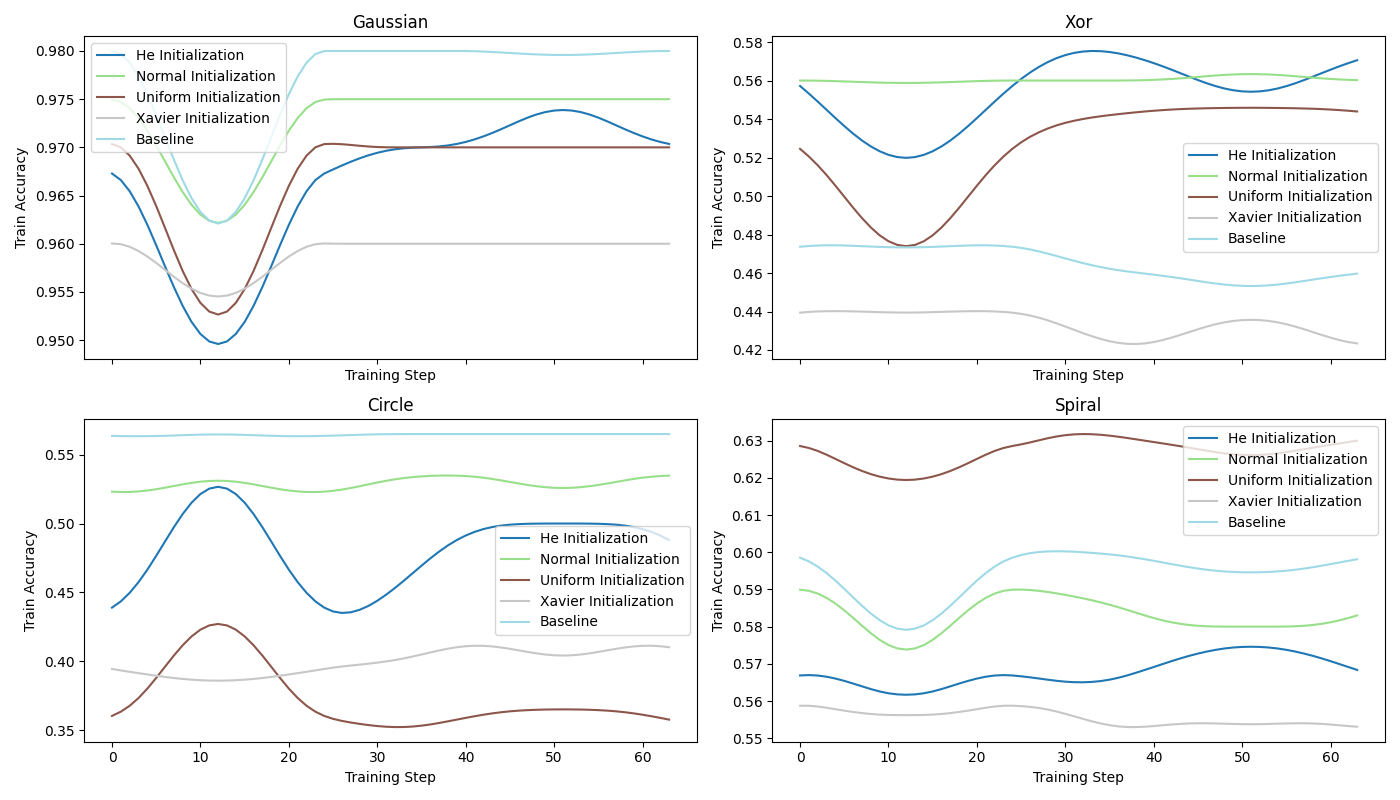
\includegraphics[width=\textwidth]{train_acc.png}
    \caption{Training accuracy over time for each dataset across different initialization strategies.}
    \label{fig:train_acc}
\end{figure}

\subsection{Decision Boundaries}
Figure \ref{fig:decision_boundaries} visualizes the decision boundaries learned by the neural network for each dataset across different initialization strategies. The contour plots show the decision boundaries, and the scatter plots show the actual data points. The title of each subplot includes the test accuracy for that particular combination of dataset and initialization strategy.

\begin{figure}[h]
    \centering
    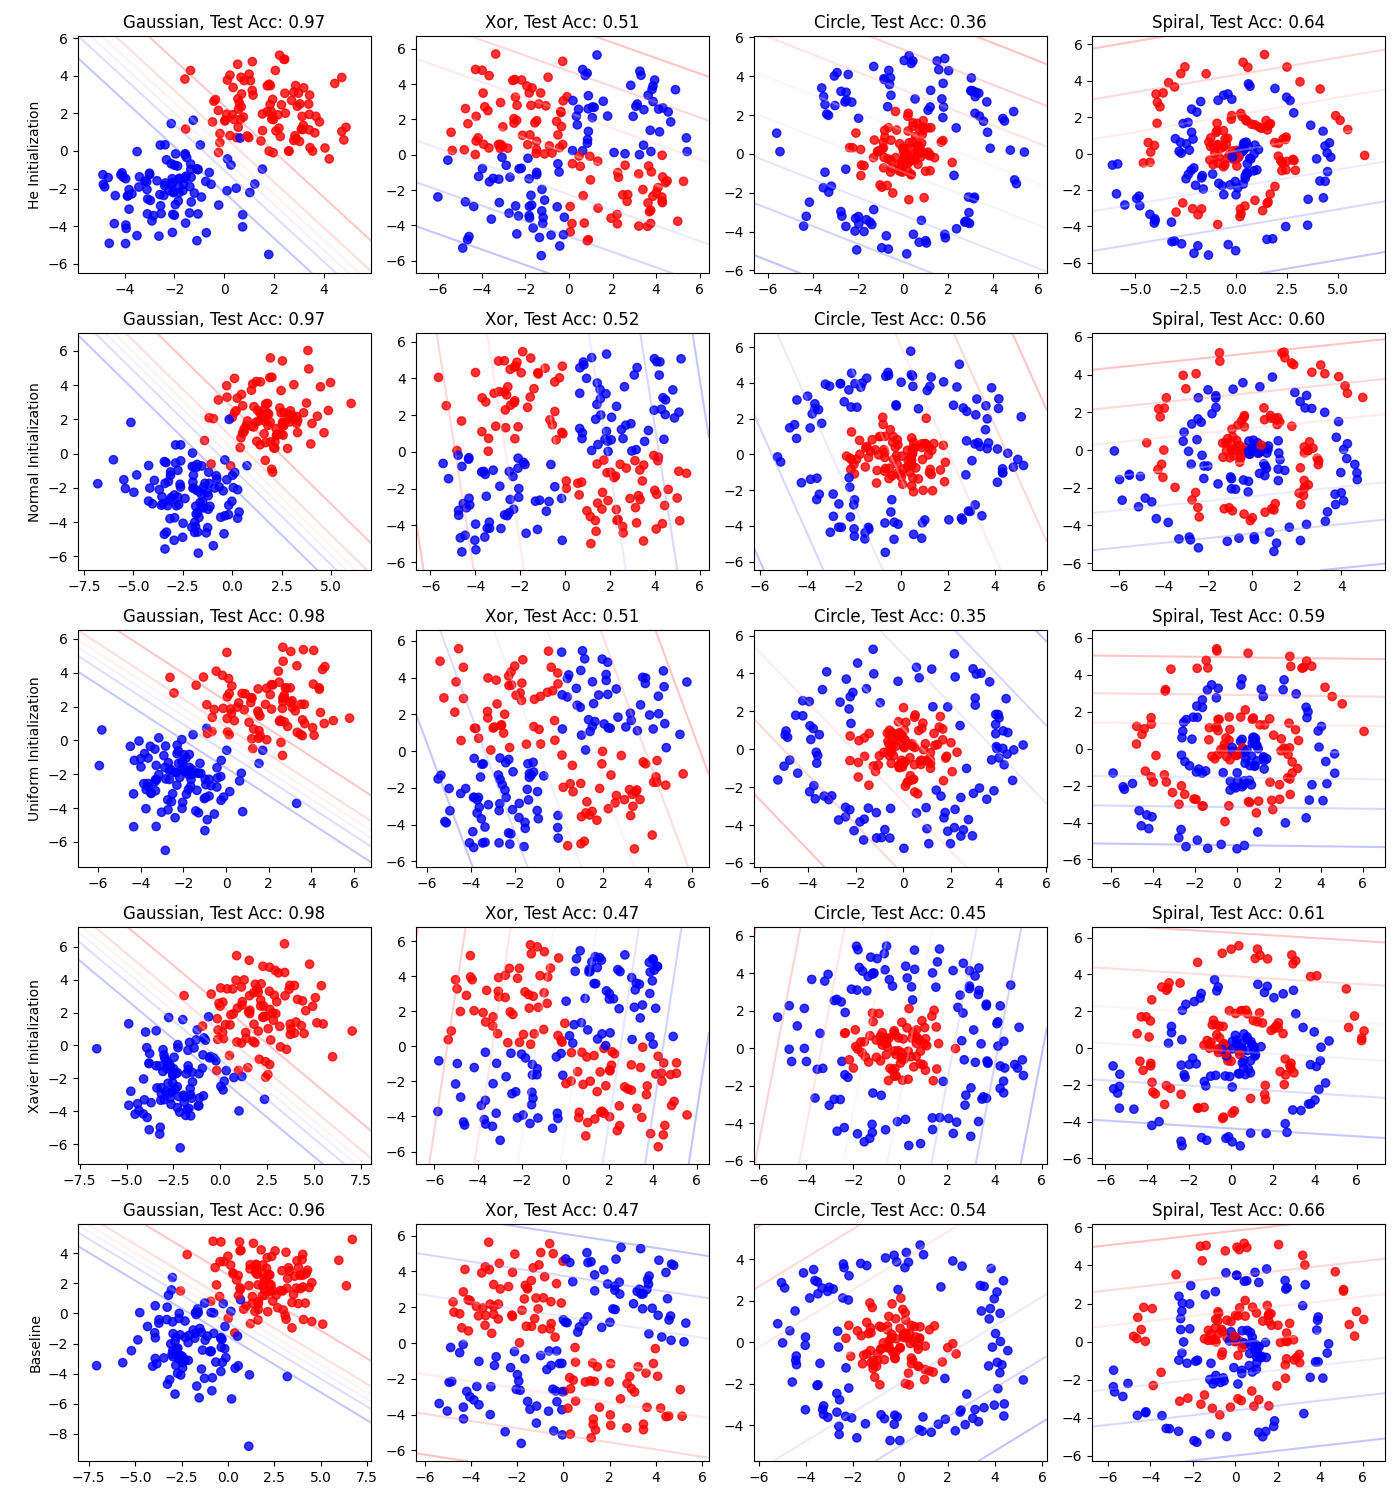
\includegraphics[width=\textwidth]{generated_images.png}
    \caption{Decision boundaries learned by the neural network for each dataset across different initialization strategies.}
    \label{fig:decision_boundaries}
\end{figure}

\subsection{Limitations}
While our results provide valuable insights into the impact of weight initialization strategies, there are several limitations to our study. First, we only evaluated a limited set of datasets and initialization strategies. Future work could explore additional datasets and more advanced initialization methods. Second, our experiments were conducted on a standard computing environment without hardware accelerations, which may limit the scalability of our approach. Finally, we did not investigate the interaction between weight initialization and other training techniques, such as batch normalization and advanced optimization algorithms, which could further enhance our understanding of neural network training dynamics.

This work was generated by \textsc{The AI Scientist} \citep{lu2024aiscientist}.

\section{Conclusions and Future Work}
\label{sec:conclusion}

In this paper, we explored the impact of various weight initialization strategies on neural networks trained using error diffusion learning. We implemented and evaluated several methods, including Xavier, He, uniform random, and normal distribution, across four datasets: XOR, Gaussian, spiral, and circle. Our experiments provided valuable insights into the effectiveness of each strategy, guiding practitioners in selecting the most appropriate method for their applications.

Our results demonstrated that weight initialization significantly influences the training of neural networks. Xavier and normal initialization strategies showed notable improvements in accuracy and convergence speed for certain datasets, while the baseline and He initialization had mixed results. The Gaussian dataset consistently achieved high accuracy across all strategies, highlighting its suitability for evaluating initialization methods. In contrast, the XOR dataset posed a greater challenge, with only normal initialization showing a notable improvement.

Despite the valuable insights gained, our study has several limitations. We evaluated a limited set of datasets and initialization strategies, and our experiments were conducted on a standard computing environment without hardware accelerations. Additionally, we did not explore the interaction between weight initialization and other training techniques, such as batch normalization and advanced optimization algorithms. These limitations suggest several avenues for future research.

Future work could extend our study by exploring additional datasets and more advanced initialization methods. Investigating the effects of weight initialization in conjunction with other training techniques, such as batch normalization \citep{ba2016layer} and advanced optimization algorithms \citep{loshchilov2017adamw}, could provide a deeper understanding of neural network training dynamics. Furthermore, evaluating the impact of initialization strategies on more complex architectures and larger datasets would enhance the generalizability of our findings.

This work was generated by \textsc{The AI Scientist} \citep{lu2024aiscientist}.

\bibliographystyle{iclr2024_conference}
\bibliography{references}

\bibliographystyle{iclr2024_conference}
\bibliography{references}

\end{document}
